
%     %%%%%%%%%%%%%%%
%
%     P A C K A G E S
%
%     %%%%%%%%%%%%%%%

\documentclass[11pt, a4paper]{article}
\usepackage{fontspec}
\usepackage{caption}
\usepackage{mathtools}
\usepackage{gensymb}

% DOCUMENT LAYOUT
\usepackage{geometry}
\geometry{a4paper, textwidth=42em, textheight=70em, marginparsep=0.5em, marginparwidth=3.5em}
\setlength\parindent{0em}
\setlength\parskip{0.75em}
\captionsetup{width=0.8\textwidth}

% FONTS
\usepackage[usenames,dvipsnames]{xcolor}
\usepackage{xunicode}
\usepackage{xltxtra}
\defaultfontfeatures{Mapping=tex-text}
%\setromanfont [Ligatures={Common}, Numbers={OldStyle}, Variant=01]{Linux Libertine O}
%\setmonofont[Scale=0.8]{Monaco}
%%% modified by Karol Kozioł for ShareLaTeX use
\setmainfont[
  Ligatures={Common}, Numbers={OldStyle}, Variant=01,
  BoldFont=LinLibertine_RB.otf,
  ItalicFont=LinLibertine_RI.otf,
  BoldItalicFont=LinLibertine_RBI.otf
]{LinLibertine_R.otf}
\setmonofont[Scale=0.8]{DejaVuSansMono.ttf}

% HEADINGS
\usepackage{sectsty}
\usepackage[normalem]{ulem}
\sectionfont{\mdseries\upshape\Large}
\subsectionfont{\mdseries\scshape\normalsize}
\subsubsectionfont{\mdseries\upshape\normalsize}

\renewenvironment{abstract}{%
{\mdseries\scshape\Large\abstractname}
\vspace{1em}\\
}{\par\noindent}


\usepackage[superscript]{cite}

% LISTINGS
\usepackage{listings}
\usepackage{color}
\usepackage{appendix}

\usepackage{color}
\definecolor{codered}{rgb}{0.61,0.21,0.18}
\definecolor{codegreen}{rgb}{0,0.6,0}
\definecolor{codegray}{rgb}{0.5,0.5,0.5}
\definecolor{codepurple}{rgb}{0.58,0,0.82}
\definecolor{backcolour}{rgb}{1.0,1.0,1.0}
\lstset{
  backgroundcolor=\color{backcolour},   
  commentstyle=\color{codegray},
  keywordstyle=\color{codered},
  numberstyle=\tiny\color{codegreen},
  stringstyle=\color{codepurple},
  basicstyle=\footnotesize\ttfamily,        % the size of the fonts that are used for the code
  breaklines=true,                          % sets automatic line breaking
  keepspaces=true,                          % keeps spaces in text, useful for keeping indentation of code
  showspaces=false,                         % show spaces everywhere adding particular underscores; it overrides 'showstringspaces'
  showstringspaces=false,                   % underline spaces within strings only
  showtabs=false,                           % show tabs within strings adding particular underscores
  stepnumber=2,                             % the step between two line-numbers. If it's 1, each line will be numbered
  tabsize=4, 	                            % sets default tabsize to 2 spaces
  title=\lstname                            % show the filename of files included with \lstinputlisting
}


%     %%%%%%%%%%%%%%%
%
%     D O C U M E N T
%
%     %%%%%%%%%%%%%%%


\begin{document}
\title{IAR Task 2 Report}
\author{Angus Pearson -- s1311631\\ Jevgenij Zubovskij -- s1346981}
\date{\today}
\maketitle

%       ^v^v^v^v^v^v^v^v^v^v^v^v^v^v^v^v^v^v^v^v^v^v^v^v^v^v^v^v^v^v^v^v^v^v^v^


\begin{abstract}
  % TODO : Maybe do more experiments?
  We present an implementation of an algorithm similar to \textit{Bug2} \cite{principlesrobot} 
  built atop reactive obstacle collision avoidance and edge following behaviour developed for 
  \textit{Task1}. The existing architecture is extended to include storing and publishing 
  timestamped poses and goal states in a Redis \cite{Redis} server.
  Real-time visualisation using a Redis to ROS \cite{ROS} pipe provides a graphical display 
  of odometry, sensory information and goals in Rviz. After-the-fact plotting is provided 
  with MatPlotLib independent of ROS.

  In our testing, the robot was able to navigate to within 10cm of the origin (it's start point) 
  from an abitary location in multiple environments successfully in 12/15 experiments, where each 
  environment was designed to evoke edge-case behaviour considered hard for the algorithm. The 
  algorithm performs comparably in a static world and a dynamic one in which other actors 
  (e.g. Humans) present a transient obstacle. 
\end{abstract}

%       ^v^v^v^v^v^v^v^v^v^v^v^v^v^v^v^v^v^v^v^v^v^v^v^v^v^v^v^v^v^v^v^v^v^v^v^


\section{Introduction}
\label{Introduction}

The second IAR assignment entails extending the existing systems from Task 1 with Odometry, 
to maintain an estimate of the robot's location, enabling rendering of it's movement both 
in real time and after reaching the goal. The task also calls for `return to home' ability, 
``either by retracing its outward route or more directly''. As an extention, basic mapping 
of the world is desireable (without localisation correction for odometry dead-reckoning drift). 

The navigational behaviour we have developed is bolted-on to the simpler reactive wall-following
and collision avoidance code we have from \textit{Task1}, in a hybrid-subsumtive sense where the
higher-level return navigation generally informs the Robot's behaviour, but if proximity thresholds
are violated the lower level reaction will peturb the trajectory away from an obstacle until the
error clears.

We use Rviz for real-time plotting, a popular graphical tool for ROS to live-render the Khepera 
Robot's pose, odometry trail, obstacles perceived by the IR range sensors and goal (a plan-line 
to the origin). Rviz is plotting standard ROS messages we publish to `topics', such as Poses,
Paths and Point Clouds.


%       ^v^v^v^v^v^v^v^v^v^v^v^v^v^v^v^v^v^v^v^v^v^v^v^v^v^v^v^v^v^v^v^v^v^v^v^


\section{Odometry}
\label{Odometry}


The goal of odometry was to find the global pose of the robot ${(X,Y,\Theta)}$. It was decided
to use the strarting position of the robot as the origin of the coordinate system ${(0, 0)}$ 
and the forward-facing direction of the robot as the positive direction of the X-axis and
all angles are measured in relation to that. We also need to account for odometry drifting with
time due to wheel slippage, non-ideal encoders as well as approximations used in calculations etc.

Moreover, we assume that the wheels have equal diameter and therefore that the data given in the 
Khepera 2 User Manual \cite{khepera_manual} is correct and an increment of 12 encoder ticks 
means a wheel has driven 1mm in that direction. 

The advantage of the Khepera is that it has very thin wheels, meaning almost a single point of contact
to the floor, which make odometry much more accurate.

\subsection{Research}

Before settling on a method to use, we researched several papers and websites for inspiration or 
already fully conceptualized solutions or even a fully developed and tested approach. The first one
we found used a fourth order Runge-Kutta numerical integrator \cite{runge_kutta} and looked like 
it would compensate for non-ideal encoders. However, upon implementation, and  testing if it correctly 
detects the robot going in a straight line (equal motor speeds) and said algorithm absolutely fialing,
it was abandoned. 

Hence, a very simple yet mathematically sound approach \cite{odo_used} was adapted 



\subsection{Method Chosen}

The method chosen for calculating pose\cite{odo_used} use simple trigonometry and differential drive on 
the wheels to perform its task. Please see the relevant document for deriviation of the formulas. The position for 
(X,Y,$\Theta$) are in in relation to initial position, where the forward-facing direction is the positive half of the
X-axis and initial X,Y are ($0$,$0$) and therefore further angles are in that frame of reference.

\begin{enumerate}

	\item Distance driven by each wheel $\Delta s_{wheel} = \frac {\Delta ticks_{wheel} } {12 ^{ticks}/_{mm}} $
	\item Total distance driven $ \Delta s = \frac{\Delta s_{r} + \Delta s_{l} }{2}$
	\item Direction in which it was driven (and new orientation) $\Theta s = \frac{ \Delta s_{r} - \Delta s_{l} }{2L}$ where L is the wheel base 
	(distance between points of contact of the two wheels to the floor)
	\item X position update $X_{n+1} = X_{n} + \Delta s \cos (\Theta)$
	\item Y position update $Y_{n+1} = Y_{n} + \Delta s \sin (\Theta)$


\end{enumerate}


The distance driven by each wheel is not as per document we mainly used as we know 
how many (encoder) ticks are per milimeter. The method proved very sucessful as 
will be shown in subsequent sections. The encoders are incremental and are able to 
detect both forward and backward movement of the wheel, hence, the above method works 
without any tricks.

\subsection{Calibration}

TODO ... take a pic of a fuckign square box.......

The odometry was initially tested in a square box to see if it detects $90$\degree turns correctly 
(while following the walls of the box) as well as distances. Initially it did not, however, we 
found multiple mobile robot odometry calibration articles and used one of them\cite{odo_calibration}
 to calibrate our Khepera. As shown, we reduced the wheelbase if the angle was shown to be too small 
and increased if it was too large until we saw that the odometry detected the  $90$\degree turns correctly. 
Hence, the actual $5$ cm wheelbase is $5.6$ cm in the code.

Hence, odometry development was finished, the code was modularly isolated from the navigation algorithm 
into corresponding state data structures (please see code). For more detailed testign see 
\textit{\S\ref{Testing Odometry} Testing Odometry}


%       ^v^v^v^v^v^v^v^v^v^v^v^v^v^v^v^v^v^v^v^v^v^v^v^v^v^v^v^v^v^v^v^v^v^v^v^


\section{Plotting}
\label{Plotting}

The control logic for the robot generates an estimated Pose at each iteration, realtive to the 
Robot's starting location (i.e. the origin). In addition to poses, which can be chained to 
form an odometry trail, it is useful to plot a Goal Line, which is the straight line the 
Return Algorithm plans to take to reach the origin. For illustrative purposes, we also render
a Point Cloud generated from the Khepera's eight IR sensors, transformed from activations
to distances in the Robot's frame of reference.

\begin{figure}[h]
  \begin{center}
    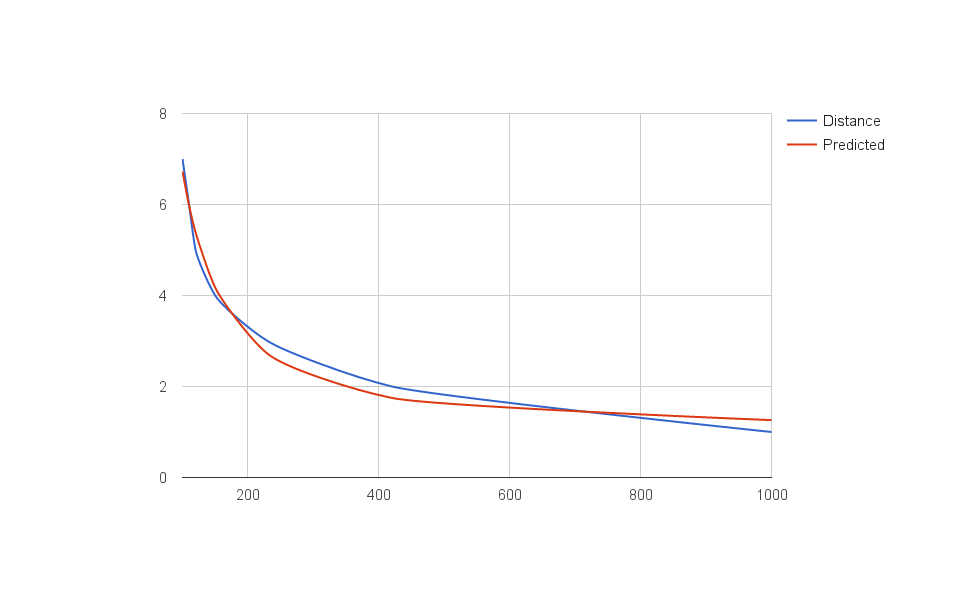
\includegraphics[width=32em]{../assets/plots/sensor-equation.png}
  \end{center}
  \begin{equation}
    S = 1.074519 + 
    \frac{9.502961}
         {(1 + \frac{\alpha}{70.42612}^{69.9039})^{0.02119919}}
  \end{equation}
  \caption{Solved equation translation betweek $S$, the distance, and $\alpha$, 
    the raw activation data of the sensor.}
\end{figure}


%       ^v^v^v^v^v^v^v^v^v^v^v^v^v^v^v^v^v^v^v^v^v^v^v^v^v^v^v^v^v^v^v^v^v^v^v^

\section{Return Algorithm}
\label{Return Algorithm}

Since Task 2 only mentions odometry and mapping is only mentioned in Task 3, we assumed that we should
be able to return to the start position of the robot ($0$,$0$) (the goal) with using only IR sensors for avoiding obstacles
and odometry for pose calculations. 

\subsection{Research}

Through researhing for algorithms that would only use the end (and knowing the current) position for navigation, 
found the so called Bug algorithms as the are insect inspired. Bug 2 is the robuts and 
(on average) the most efficient out of the three mentioned bug algorithms. 
Hence, it was chosen to be implemented.


\subsection{Method Chosen}

TODO .... insert picture from document


The Bug 2 algorithms is quite easy conceptually. The assumptions it needs to work properly can be simplified to:

\begin{enumerate}

	\item Known direction to goal and robot can measure distance between points
	\item Be in a bounded workspace with a finite number of finitie size objects

\end{enumerate}

Hence, we satisfy these assumptions by having odometry and a global frame of reference as well 
as a square box arena with physical obstacles.

The algorithm is:

\begin{enumerate}

	\item Head toward goal on the m-line
	\item if an obstacle is in the way, follow it until you encounter the m-line again closer to the goal
	\item Leave the obstacle and continue toward the goal

\end{enumerate}

\subsection{Needed Alterations}

However, the implementation is much less trivial than the higher level description. It it had 
to be altered due to problems that became evident during testing (please see \textit{Testing Return Algorithm}).

\subsubsection{Thresholding}

the first problem is that due to imperfect encoders, wheel slippage, odometry drift as well as not
beign able to sample odometry more often than every $20$ ms\cite{khepera_manual} (due to sequential 
reads of IR being in the same loop. Moreover, one must remember odometry fomulas used are only approximations.

Hence, all odometry and position-related calculations can not be strict equalities to compensate 
for the error the above introduces. Hence, all values are considered "on-point" as long as the 
fall within $\pm$ threshold of ideal value. Some thresholds are several centimeters.

\subsubsection{M-line Replanning}


Testing also revealed that about $1/15$ times the claculations of the approach angle to the goal would 
fail and be 180 \degree more than the real value. Many attampts were made to trace down the bug, however,
none were successful. Hence, we made an alteration to the Bug 2, so if it is in free space (not following 
walls or beign "unstuck"\cite{task1_report} and it goes away from the last detected m-line segment for more
than a threshold value, we recompute the approach vector to the goal.

This revealed another bug that was left over from task 1 as in the wall following was state-based and sometimes
a spike in sensor readings made it seem that the tobot left the wall and was in free space, recomputing the M-line
wrongly even if it continued to follow the wall. 


This was countered by introducing another distance check into the Bug algorithm, to check if we could still 
theoretically follow the wall, in which case the threshold at which we would recompute the M-line was several 
times larger than the one for recom[uting in free space. Hence, even if robot gets stuck in a particular scenarion, 
there should be very few edge cases wher it will get trapped and continue reocmputing the M-line, getting itself stuck again.
Altering the two constants for M-line recomputing is what was also done durting testing to minimize said edge cases.


%       ^v^v^v^v^v^v^v^v^v^v^v^v^v^v^v^v^v^v^v^v^v^v^v^v^v^v^v^v^v^v^v^v^v^v^v^

\section{Testing Plotting}
\label{Testing Plotting}


%       ^v^v^v^v^v^v^v^v^v^v^v^v^v^v^v^v^v^v^v^v^v^v^v^v^v^v^v^v^v^v^v^v^v^v^v^


\section{Testing Odometry}
\label{Testing Odometry}


%       ^v^v^v^v^v^v^v^v^v^v^v^v^v^v^v^v^v^v^v^v^v^v^v^v^v^v^v^v^v^v^v^v^v^v^v^



\section{Testing Return Algorithm}
\label{Testing Return Algorithm}



%       ^v^v^v^v^v^v^v^v^v^v^v^v^v^v^v^v^v^v^v^v^v^v^v^v^v^v^v^v^v^v^v^v^v^v^v^

\section{Experimental Results}
\label{Results}


\section{Discussion \& Possible Improvements}
\label{Discussion}


%       ^v^v^v^v^v^v^v^v^v^v^v^v^v^v^v^v^v^v^v^v^v^v^v^v^v^v^v^v^v^v^v^v^v^v^v^

\newpage
\begin{thebibliography}{8}

\bibitem{principlesrobot}
\par{Principles of Robot Motion: Theory, Algorithms, and Implementation \S2.1}\\
\textit{Howie Choset}

\bibitem{Redis}
\par{Redis is an open source (BSD licensed), in-memory data structure store, used as database, cache and message broker. It supports data structures such as strings, hashes, lists, sets, sorted sets with range queries, bitmaps, hyperloglogs and geospatial indexes with radius queries.}\\
\textit{http://redis.io}

\bibitem{ROS}
\par{The Robot Operating System (ROS) is a flexible framework for writing robot software. It is a collection of tools, libraries, and conventions that aim to simplify the task of creating complex and robust robot behavior across a wide variety of robotic platforms.}\\
\textit{http://www.ros.org/}

\bibitem{runge_kutta} 
\par{Fourth order Runge - Kutta algorithm for pose estimation} \\
\textit{https://www.cs.cmu.edu/afs/cs.cmu.edu/academic/class/16311/www/s07/labs/NXTLabs/Lab\%203.html }

\bibitem{odo_used} 
\par{Princeton University lecture on Autonomous Robot Navigation with odometry formulas and their deriviation from geometry and trigonometry. These formulas are devised specifically for differential drive robots} \\
\textit{https://www.cs.princeton.edu/courses/archive/fall11/cos495/COS495-Lecture5-Odometry.pdf }

\bibitem{odo_calibration} 
\par{The Technic Gear website article dealign with differential drive robot odometry calculations} \\
\textit{http://thetechnicgear.com/2014/06/howto-calibrate-differential-drive-robot/}

\bibitem{khepera_paper} 
\par{A paper on Experimental Odometry Calibration of the Mobile Robot Khepera II Based on the Least-Squares Technique from which we took inspiration on calibration and confirmation we are doing odometry in the right fashion} \\
\textit{http://ieeexplore.ieee.org/stamp/stamp.jsp?arnumber=1570321}


\bibitem{khepera_manual} 
\par{Khepera 2 user Manual containing all the fundamental information about the Khepera 2 robot, including information abotu encoders and their value meanings} \\
\textit{http://ftp.k-team.com/khepera/documentation/Kh2UserManual.pdf}


\bibitem{taske1_report} 
\par{Our Task1 solution and report} \\
\textit{Angus Pearson, Jevgenij Zubovskij}





\end{thebibliography}


\begin{appendices}
\section*{Appendix}
\subsection{Code Listings}
\lstinputlisting[language=python]{../../main.py}
\lstinputlisting[language=python]{../../data.py}
\lstinputlisting[language=python]{../../state.py}
\lstinputlisting[language=python]{../../bug_state.py}
\lstinputlisting[language=python]{../../bug_algorithm.py}
\lstinputlisting[language=python]{../../navigation_algorithm.py}
\lstinputlisting[language=python]{../../odometry_algorithm.py}
\lstinputlisting[language=python]{../../odometry_state.py}
\lstinputlisting[language=python]{../../constants.py}
\end{appendices}


\end{document}
